\documentclass[10pt,foldmark]{leaflet}
\renewcommand*\foldmarkrule{.3mm}
\renewcommand*\foldmarklength{5mm}
\usepackage[italian]{babel}
\usepackage[utf8]{inputenc}
\usepackage[T1]{fontenc}

\usepackage{graphicx}
\usepackage{amsmath}
\usepackage{textcomp}
\usepackage{mathptmx}
\usepackage[scaled=0.9]{helvet}
\usepackage{lipsum}
\usepackage{mhchem}
\usepackage{subfigure}

\usepackage[dvipsnames,usenames]{color}
\definecolor{LIGHTGRAY}{gray}{.9}

%%%%\renewcommand{\descfont}{\normalfont}
%\newcommand\Lpack[1]{\textsf{#1}}
%\newcommand\Lclass[1]{\textsf{#1}}
%\newcommand\Lopt[1]{\texttt{#1}}
%\newcommand\Lprog[1]{\textit{#1}}

\newcommand*\defaultmarker{\textsuperscript\textasteriskcentered}

\newcommand{\doppiobeta}{$ 0\nu\beta\beta$}
\newcommand{\geant}{Geant4}

%\title{\bf Carolina Dynamics Symposium}

%\author{%
%\Large \bf Clemson University
%  Martin Schmoll\\
%  Predrag Puno\v{s}evac
%}
%\date{\bf April 13 -- April 15, 2012 }

%\CutLine*{1}% Dotted line without scissors
%\CutLine*{6}% Dotted line without scissors

%\CutLine{6}%  Dotted line with scissors

%\AddToBackground{1}{%  Background of a small page
%  \put(0,0){\textcolor{Cerulean}{\rule{\paperwidth}{\paperheight}}}}


%\AddToBackground{1}{%  Background of a small page
%  \put(40,200){\includegraphics[scale=0.04]{numen_logo.jpeg}}}


%\AddToBackground{6}{%  Background of a small page
%  \put(0,0){\textcolor{YellowOrange}{\rule{\paperwidth}{\paperheight}}}}


%\AddToBackground*{2}{% Background of a large page
%  \put(\LenToUnit{.5\paperwidth},\LenToUnit{.5\paperheight}){%
%    \makebox(0,0)[c]{%
%      \resizebox{.9\paperwidth}{!}{\rotatebox{35.26}{%
%        \textsf{\textbf{\textcolor{LIGHTGRAY}{CLEMSON}}}}}}}}

%\AddToBackground*{1}{% Background of a large page
%  \put(\LenToUnit{.66\paperwidth},\LenToUnit{.36\paperheight}){%
%    \makebox(0,0)[c]{%
%      \resizebox{.3\paperwidth}{!}{\rotatebox{0.0}{%
%        \includegraphics{numen_logo.jpeg} }}}}}


\begin{document}

\begin{center}
%\includegraphics[width=16em]{unict_dfa}\\
%\uppercase{Universit\`a degli Studi di Catania}\\
%{\sc dipartimento di fisica e astronomia}\\
%{\sc corso di laurea triennale in fisica}\\
\begin{minipage}[c]{0.45\textwidth}
\begin{flushleft}

\includegraphics[width=0.8\textwidth]{logo_unict_orizzontale}
\end{flushleft}
\end{minipage}
\hfill
\begin{minipage}[c]{0.45\textwidth}
\begin{flushright}

\includegraphics[width=\textwidth]{logo_dfa_orizzontale}
\end{flushright}
\end{minipage}\\
\medskip
{\sc corso di laurea magistrale in fisica}\\
\hbox to \textwidth{\hrulefill}

\vspace{3truecm}

{\sc Giuseppe Antonio Brischetto}

\vfill

\uppercase{\sc Simulazioni Monte Carlo di un sistema di rivelazione per ioni pesanti basato sulla tecnologia SiC-CsI per il progetto NUMEN}

\vfill

\centerline{\hbox to 3.5truecm{\hrulefill}}
{\sc elaborato finale}\\
%{\sc tesi di laurea}\\
\centerline{\hbox to 3.5truecm{\hrulefill}}

\vfill

\begin{minipage}{\textwidth}
\begin{flushright}
\begin{minipage}{0.3\textwidth}
\begin{tabbing}
Chiar.mo \= Prof. P. Pallino \kill
Relatore: \> \\
Chiar.mo \> Prof. F. Cappuzzello \\
\\
\textsc{Correlatore:} \\
\textsc{Dott. L. Pandola}
\end{tabbing}
\end{minipage}
\end{flushright}
\end{minipage}

\vfill

\hbox to \textwidth{\hrulefill}
{\sc anno accademico 2018/2019}

\end{center}

\newpage

\section{Abstract}

%\lipsum[1]
%Questo lavoro di tesi verte sulla realizzazione di un tool di simulazioni Monte Carlo per lo studio di un sistema di rivelazione basato sulla tecnologia SiC-CsI per l'identificazione di ioni pesanti nell'ambito del progetto NUMEN.
%Tale progetto propone ai Laboratori Nazionali del Sud un nuovo metodo per estrarre dai dati sperimentali informazioni sugli elementi di matrici nucleare che entrano in gioco nel tempo di dimezzamento del doppio decadimento beta senza neutrini.
Il progetto NUMEN ha recentemente promosso ai Laboratori Nazionali del Sud un'importante ristrutturazione verso alte correnti di fascio del Ciclotrone Superconduttore K800 e dello spettrometro magnetico MAGNEX.
L'upgrade di MAGNEX prevede l'introduzione di un muro di telescopi $\Delta E - E$ a stato solido, basato sulla tecnologia SiC-CsI, per l'identificazione di ioni pesanti ad alto rate.
Questo lavoro di tesi verte sulla realizzazione di un tool di simulazioni Monte Carlo per lo studio e l'ottimizzazione di tale sistema di rivelazione.
%Il tool è stato sviluppato e implementato integrando i software per la ricostruzione del moto dei prodotti di reazione attraverso lo spettrometro con un'applicazione specifica basata sulla piattaforma \geant.
Uno degli obiettivi di questo lavoro consiste nella valutazione delle prestazioni del sistema simulato in termini di capacità di identificazione degli ioni di interesse, rapporto segnale-rumore e sensibilità di misura.
%In particolare, tale tool è stato utilizzato per valutare le prestazioni del sistema simulato in termini di capacità di identificazione degli ioni di interesse, rapporto segnale-rumore e sensibilità di misura, nonché per ottimizzare le condizioni di granularità dei telescopi.
In aggiunta, il tool è stato utilizzato per ottimizzare la granularità dei~telescopi.



\begin{figure} [!h]
	\centering
	\includegraphics[width=0.8\columnwidth, keepaspectratio]{Grafici/magnex_etichette.png}
\end{figure}
%\begin{center}
\hspace{0.8 cm}\textit{ Lo spettrometro magnetico MAGNEX ai LNS.}
%\end{center}


%\section{Background}
\section{Contesto scientifico}
%\lipsum[2-4]
%Nell'ultimo decennio, l'interesse suscitato dal doppio decadimento beta senza neutrini (\doppiobeta) è cresciuto senza soluzione di continuità, come testimoniano gli innumerevoli esperimenti nati per osservarlo per la prima volta; tale fenomeno rappresenta, infatti, uno strumento fondamentale per svelare alcuni dei misteri che circondano una delle particelle più elusive dell'Universo: il neutrino. 
%Il \doppiobeta{} permetterebbe non soltanto di accedere alla scala assoluta della massa del neutrino, ma anche di chiarire la sua natura fondamentale; fino ad oggi, infatti, non è noto se il neutrino è una particella di Dirac o di Majorana. 
%Inoltre, dal momento che tale fenomeno viola la conservazione del numero leptonico totale, potrebbe costituire anche la prima evidenza sperimentale di fisica oltre il Modello Standard.
%Per estrarre dagli esperimenti sul \doppiobeta{} le informazioni di interesse sul neutrino è necessario conoscere gli elementi di matrice nucleare (Nuclear Matrix Elements, NMEs) del processo di transizione del nucleo dallo stato iniziale a quello finale. 
%Tali NMEs sono finora noti soltanto per via teorica, dando luogo ad uno scenario in cui i diversi modelli mostrano tra loro sostanziali discrepanze.
%Allo scopo di risolvere queste ambiguità è nato il progetto NUMEN (NUclear Matrix Elements for Neutrinoless double beta decay), il quale propone ai Laboratori Nazionali del Sud (LNS) dell'Istituto Nazionale di Fisica Nucleare (INFN) un nuovo metodo per accedere sperimentalmente ad informazioni utili per la determinazione degli NMEs.
%Il fulcro di tale metodo è la misura di sezioni d'urto di reazioni di doppio scambio di carica (Double Charge Exchange, DCE) indotte da ioni pesanti, le quali presentano diversi aspetti in comune con il \doppiobeta.

Il progetto NUMEN (NUclear Matrix Elements for Neutrinoless double beta decay) propone ai Laboratori Nazionali del Sud (LNS) dell'Istituto Nazionale di Fisica Nucleare (INFN) un nuovo metodo per accedere sperimentalmente ad informazioni utili per la determinazione degli elementi di matrice nucleare che entrano in gioco nel tasso di dimezzamento del doppio decadimento beta senza neutrini (\doppiobeta).
Il fulcro di tale metodo è la misura di sezioni d'urto di reazioni di doppio scambio di carica (Double Charge Exchange, DCE) indotte da ioni pesanti, le quali presentano diversi aspetti in comune con il \doppiobeta.
%Essendo i processi di DCE caratterizzati da sezioni d'urto estremamente basse (tipicamente di pochi~nb), è stato finora possibile analizzare soltanto alcuni dei casi rilevanti, contraddistinti da particolari condizioni favorevoli. Tuttavia, al fine di raggiungere il suo più ambizioso obiettivo, il progetto intende studiare in modo sistematico tutti gli isotopi candidati al \doppiobeta{}. Ciò rende necessario l'utilizzo di fasci di ioni pesanti con intensità molto più elevate di quelle attualmente disponibili ai LNS. A tale scopo è stata già avviata una grande opera di ristrutturazione del Ciclotrone Superconduttore~K800 e dello spettrometro magnetico~MAGNEX.
%
%
%Poiché i processi di DCE hanno sezioni d'urto estremamente basse (tipicamente di pochi~nb), è necessario utilizzare fasci di ioni pesanti molto più intensi di quelli attualmente disponibili ai LNS.
%Per questo motivo è stata avviata una grande ristrutturazione del Ciclotrone Superconduttore~K800 e dello spettrometro magnetico~MAGNEX, alla fine della quale l'intensità disponibile sarà dell'ordine di $10^{12}$~pps: in quest'ottica, per il progetto è fondamentale lo sviluppo di tecnologie di frontiera, in grado di tollerare le correnti previste.
%
%
Dal momento che i processi di DCE hanno sezioni d'urto estremamente basse (tipicamente di pochi~nb), è stata avviata una grande opera di ristrutturazione del Ciclotrone Superconduttore~K800 e dello spettrometro magnetico~MAGNEX, per aumentare di circa due ordini di grandezza l'intensità dei fasci di ioni pesanti: in quest'ottica, per il progetto è fondamentale lo sviluppo di tecnologie di frontiera, in grado di tollerare le correnti previste.
%Alla fine dell'upgrade i fasci di ioni pesanti disponibili ai LNS avranno un'intensità dell'ordine di $10^{12}$~pps, circa due ordini di grandezza superiore a quella attuale: in quest'ottica, per il progetto è fondamentale lo sviluppo di tecnologie di frontiera, in grado di tollerare le correnti previste.
%Parte integrante di NUMEN è, dunque, un'intensa attività di ricerca e sviluppo, pertinente non soltanto al campo sperimentale ma anche a quello teorico.
%L'upgrade di MAGNEX prevede importanti cambiamenti del rivelatore di piano focale; in particolare, il progetto prevede la sostituzione del muro di rivelatori al silicio con uno di telescopi $\Delta E - E$ a stato solido, dedicato alla Particle IDentification (PID).
L'upgrade di MAGNEX prevede importanti cambiamenti del rivelatore di piano focale; in particolare, il muro di rivelatori al silicio sarà sostituito da uno di telescopi $\Delta E - E$ a stato solido, dedicato alla Particle IDentification (PID). 
Le esigenze di alta resistenza alle radiazioni hanno guidato verso la scelta di un primo stadio costituito da un rivelatore sottile (spessore 100~$\mu$m) al carburo di silicio~(SiC), seguito da un rivelatore di stop (spessore 1~cm) allo ioduro di cesio~(CsI).

\begin{figure} [!h]
	\centering
	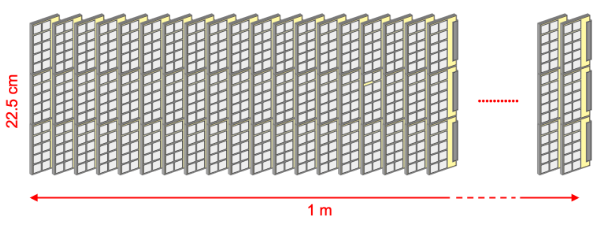
\includegraphics[width=0.88\columnwidth, keepaspectratio]{Grafici/muro_telescopi.png}
\end{figure}
%\begin{center}
\hspace{0.2 cm}\textit{Il muro di telescopi previsto dopo l'upgrade di MAGNEX.}
%\end{center}
%\section{Objectives}
\section{Obiettivi}
%\lipsum[5]
Lo scopo principale di questo lavoro di tesi consiste nello sviluppo e nell'implementazione di un tool di simulazioni per il progetto NUMEN che, per la prima volta, consenta di descrivere la cinematica di reazione, il moto degli eiettili attraverso gli elementi magnetici di MAGNEX e la loro interazione con il muro di telescopi SiC-CsI.
%All'interno di tale tool, i software dedicati al calcolo della cinematica e al trasporto ottico dei prodotti di reazione sono già esistenti e ottimizzati, mentre l'applicazione che riproduce il sistema di rivelazione è stata sviluppata nel corso di questo lavoro.
%Tale applicazione è stata realizzata utilizzando la nota piattaforma \geant{}.
Tale tool integra i software dedicati al trasporto ottico degli eiettili con una specifica applicazione \geant.
Lo sviluppo del tool è molto importante per il progetto, in quanto coinvolge aspetti legati sia alla fase di progettazione sia alla fase operativa del sistema di rivelazione.
In questo lavoro, il tool è stato utilizzato per analizzare le capacità di PID dei telescopi, calcolando il rapporto segnale-fondo e la sensibilità di misura del dispositivo.
%Esso è stato, inoltre, impiegato per ottimizzare la granularità dei telescopi.
Esso è stato, inoltre, impiegato per condurre uno studio accurato sull'ottimizzazione della granularità dei telescopi.
%Per ogni caso considerato si è stimata la frazione di eventi degradati, i quali possono costituire un fondo dal punto di vista della PID. 
%Nello studio di processi rari come quelli di DCE è, infatti, essenziale avere un'elevata sensibilità di misura delle sezioni d'urto ed un grande potere di reiezione degli eventi di fondo. 
Il lavoro svolto per questa tesi costituisce il primo passo verso lo sviluppo di una simulazione dell'intero apparato sperimentale dopo l'upgrade, che riproduca fedelmente la risposta di questo agli eventi di interesse.






%\section{Techniques}
\section{Tecniche}
%\lipsum[8]

%All'interno del tool di simulazioni, i software dedicati al calcolo della cinematica e al trasporto ottico dei prodotti di reazione sono già esistenti e ottimizzati, mentre l'applicazione che riproduce il sistema di rivelazione è stata sviluppata nel corso di questo lavoro. Tale applicazione è stata realizzata utilizzando la nota piattaforma \geant{}. Per ogni caso considerato si è stimata la frazione di eventi degradati, i quali possono costituire un fondo dal punto di vista della PID. Nello studio di processi rari come quelli di DCE è, infatti, essenziale avere un'elevata sensibilità di misura delle sezioni d'urto ed un grande potere di reiezione degli eventi di fondo. 
%Affinché le simulazioni potessero riprodurre fedelmente il comportamento reale degli ioni nello spettrometro, il tool è stato realizzato integrando tra loro due parti essenziali: la prima, dedicata alla ricostruzione della traiettoria degli ioni nello spettrometro, è costituita da software sviluppati all'uopo e ottimizzati dalla collaborazione NUMEN; la seconda, che simula l'interazione ione-rivelatore, è basata su un'applicazione scritta utilizzando la piattaforma \geant.

Le capacità di PID del telescopio SiC-CsI sono state analizzate ricostruendo, per ogni specie ionica simulata, la corrispondente matrice $\Delta E_{SiC} - E_{CsI}$, laddove $\Delta E_{SiC}$ indica la perdita di energia nel rivelatore al~SiC, mentre $E_{CsI}$ rappresenta l'energia residua rilasciata nel cristallo di~CsI.
%Le capacità di PID del telescopio SiC-CsI sono state analizzate ricostruendo, per ogni specie ionica simulata, la corrispondente matrice $\Delta E_{SiC} - E_{CsI}$.
Selezionando con un taglio grafico il luogo relativo allo ione di interesse, è stata calcolata la frazione di altri ioni inclusi in tale taglio.
I valori così ottenuti sono stati opportunamente moltiplicati per le rispettive sezioni d'urto di produzione, allo scopo di ottenere una stima delle contaminazioni reali.
Da tale stima è stato dedotto il rapporto segnale-fondo (S/B), grazie al quale è stato possibile determinare la sensibilità di misura del sistema di rivelazione.

\begin{figure} [!h]
	\centering
	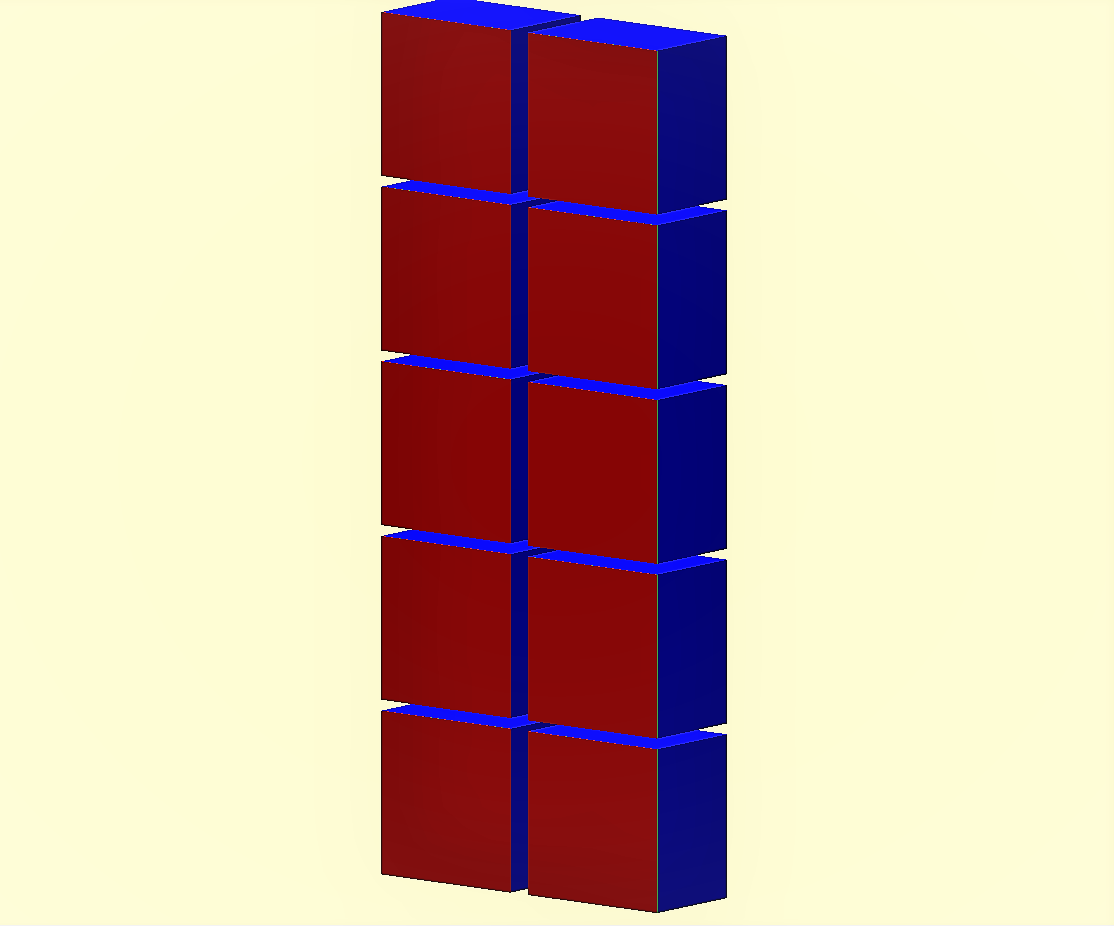
\includegraphics[width=0.5\columnwidth, keepaspectratio]{Grafici/modulo2_ritagliato.png}
\end{figure}
%\begin{center}
\textit{Geometria della simulazione \geant{} di una matrice di 2$\times$5 telescopi: in rosso il rivelatore al~SiC, in blu il cristallo di~CsI.}
%\end{center}



%\section{Results}
\section{Risultati}
%\lipsum[11]
%\includegraphics[width=0.9\columnwidth]{esempio}
%\lipsum[12-13]

Il sistema di rivelazione simulato si è dimostrato in grado di separare efficacemente gli ioni sia in numero atomico sia in numero di massa.
Si è, tuttavia, osservato che la presenza, attorno alla parte sensibile del rivelatore al~SiC, di una cornice in cui la carica prodotta dal passaggio degli ioni viene parzialmente raccolta genera degli eventi degradati, che costituiscono un fondo nella PID.
Inoltre, una seconda sorgente di fondo è rappresentata dagli ioni che, a causa dell'inclinazione della loro traiettoria, non si fermano nel cristallo di~CsI e rilasciano dunque solo una parte della loro energia residua.
Dalla simulazione è emerso che il principale contaminante allo ione di interesse~(\ce{^{20}O}) è il~\ce{^{20}F^{8+}}, originato da un processo di singolo scambio di carica.
%Alle energie di fascio considerate, la probabilità di ottenere lo stato di carica $8+$ per uno ione di \ce{^{20}F} è molto piccola; infatti, calcolando il rapporto S/B, è stato possibile dimostrare che la sensibilità di misura dell'apparato simulato nella regione di interesse è di 460~pb a 5$\sigma$, quindi adatta a misurare la reazione di~interesse.
%Le percentuali di contaminazione sono molto basse;
\begin{figure} [!t]
	\centering
	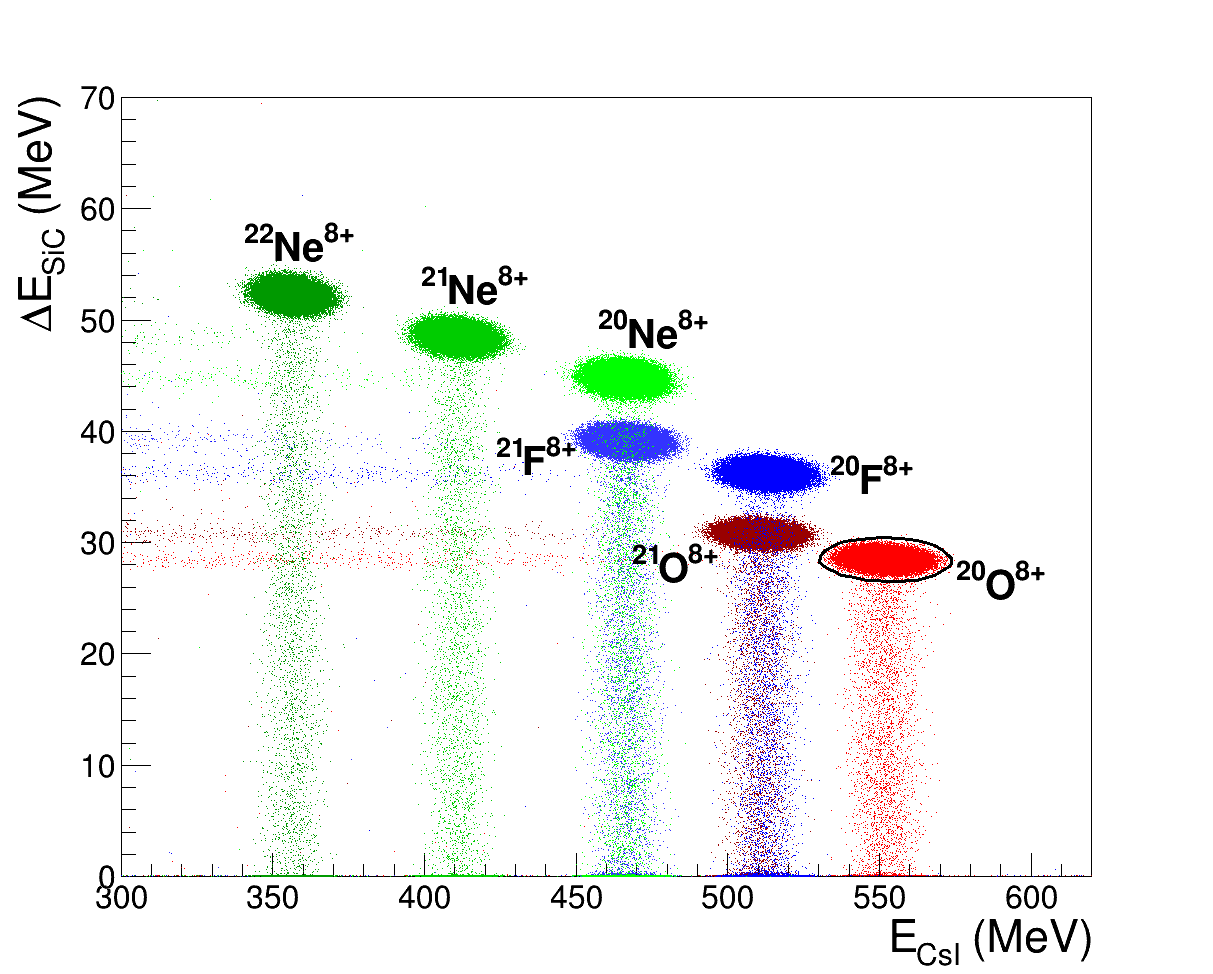
\includegraphics[width=0.7\columnwidth, keepaspectratio]{Grafici_Tesi2/PIDnew/deltaE_Ecsi_quadrata_taglio_menoeventi2.png}
\end{figure}\\
%\begin{center}
\textit{ Matrici $\Delta E_{SiC} - E_{CsI}$ con il taglio grafico per l'identificazione dello ione di interesse~(\ce{^{20}O}).}
%\end{center}
%\vspace{0.2cm}

Calcolando il rapporto S/B, la simulazione ha indicato che la sensibilità di misura dell'apparato simulato nella regione di interesse è di 460~pb a 5$\sigma$, quindi adatta a misurare la reazione di~interesse.
L'analisi di tre diverse condizioni di granularità (1$\times$1, 1.5$\times$1.5 e 2$\times$2~$\mbox{cm}^2$) ha dimostrato che, all'aumentare della superficie di rivelazione, la sensibilità di misura diminuisce, pur restando in tutti e tre i casi esaminati sufficiente per misurare il DCE.

Un aspetto fondamentale di questo lavoro è consistito nella validazione dei risultati delle simulazioni attraverso il confronto con i dati sperimentali raccolti in occasione del test con fascio accelerato svolto ad Aprile~2019.
Gli spettri energetici misurati dal rivelatore al SiC e dallo scintillatore allo CsI sono stati messi a confronto con i rispettivi spettri simulati: in entrambi i casi la compatibilità è significativa.
%\begin{figure}[h]
%	\begin{subfigure}
%		\centering
%		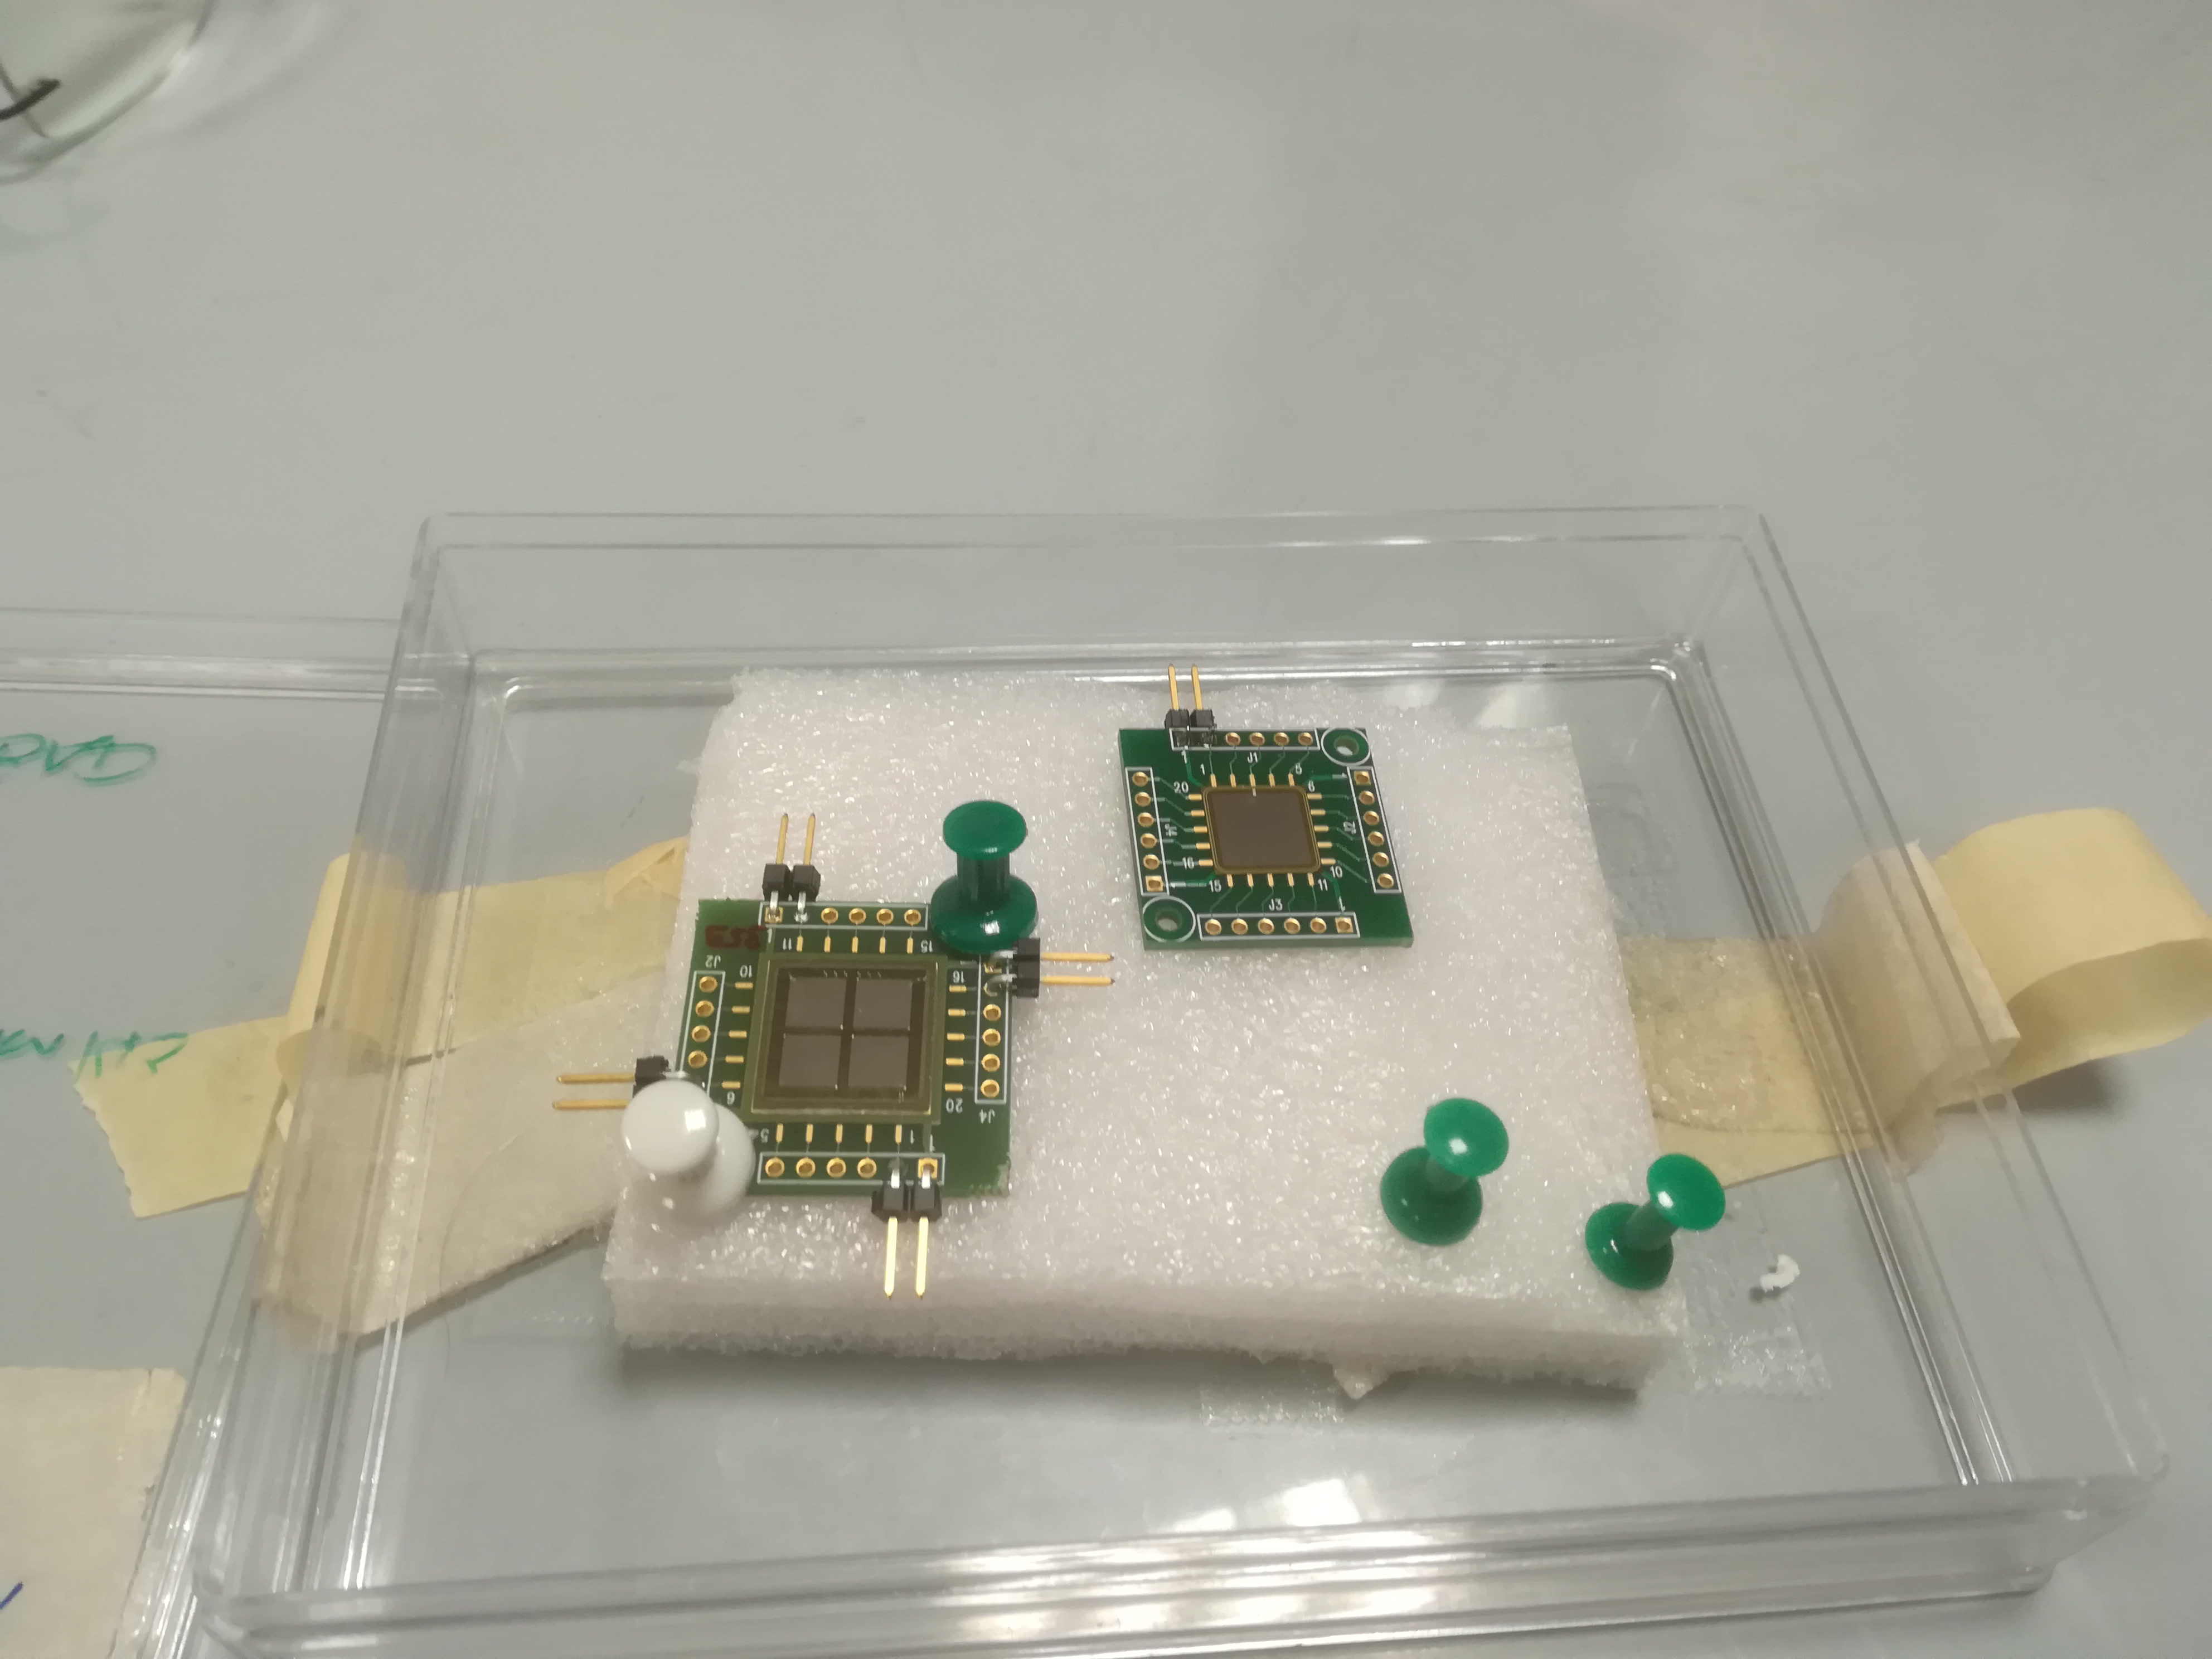
\includegraphics[width=0.48\columnwidth, keepaspectratio]{Grafici_Tesi2/Confronto/sic.png}
%	\end{subfigure}
%	\begin{subfigure}
%		\centering
%		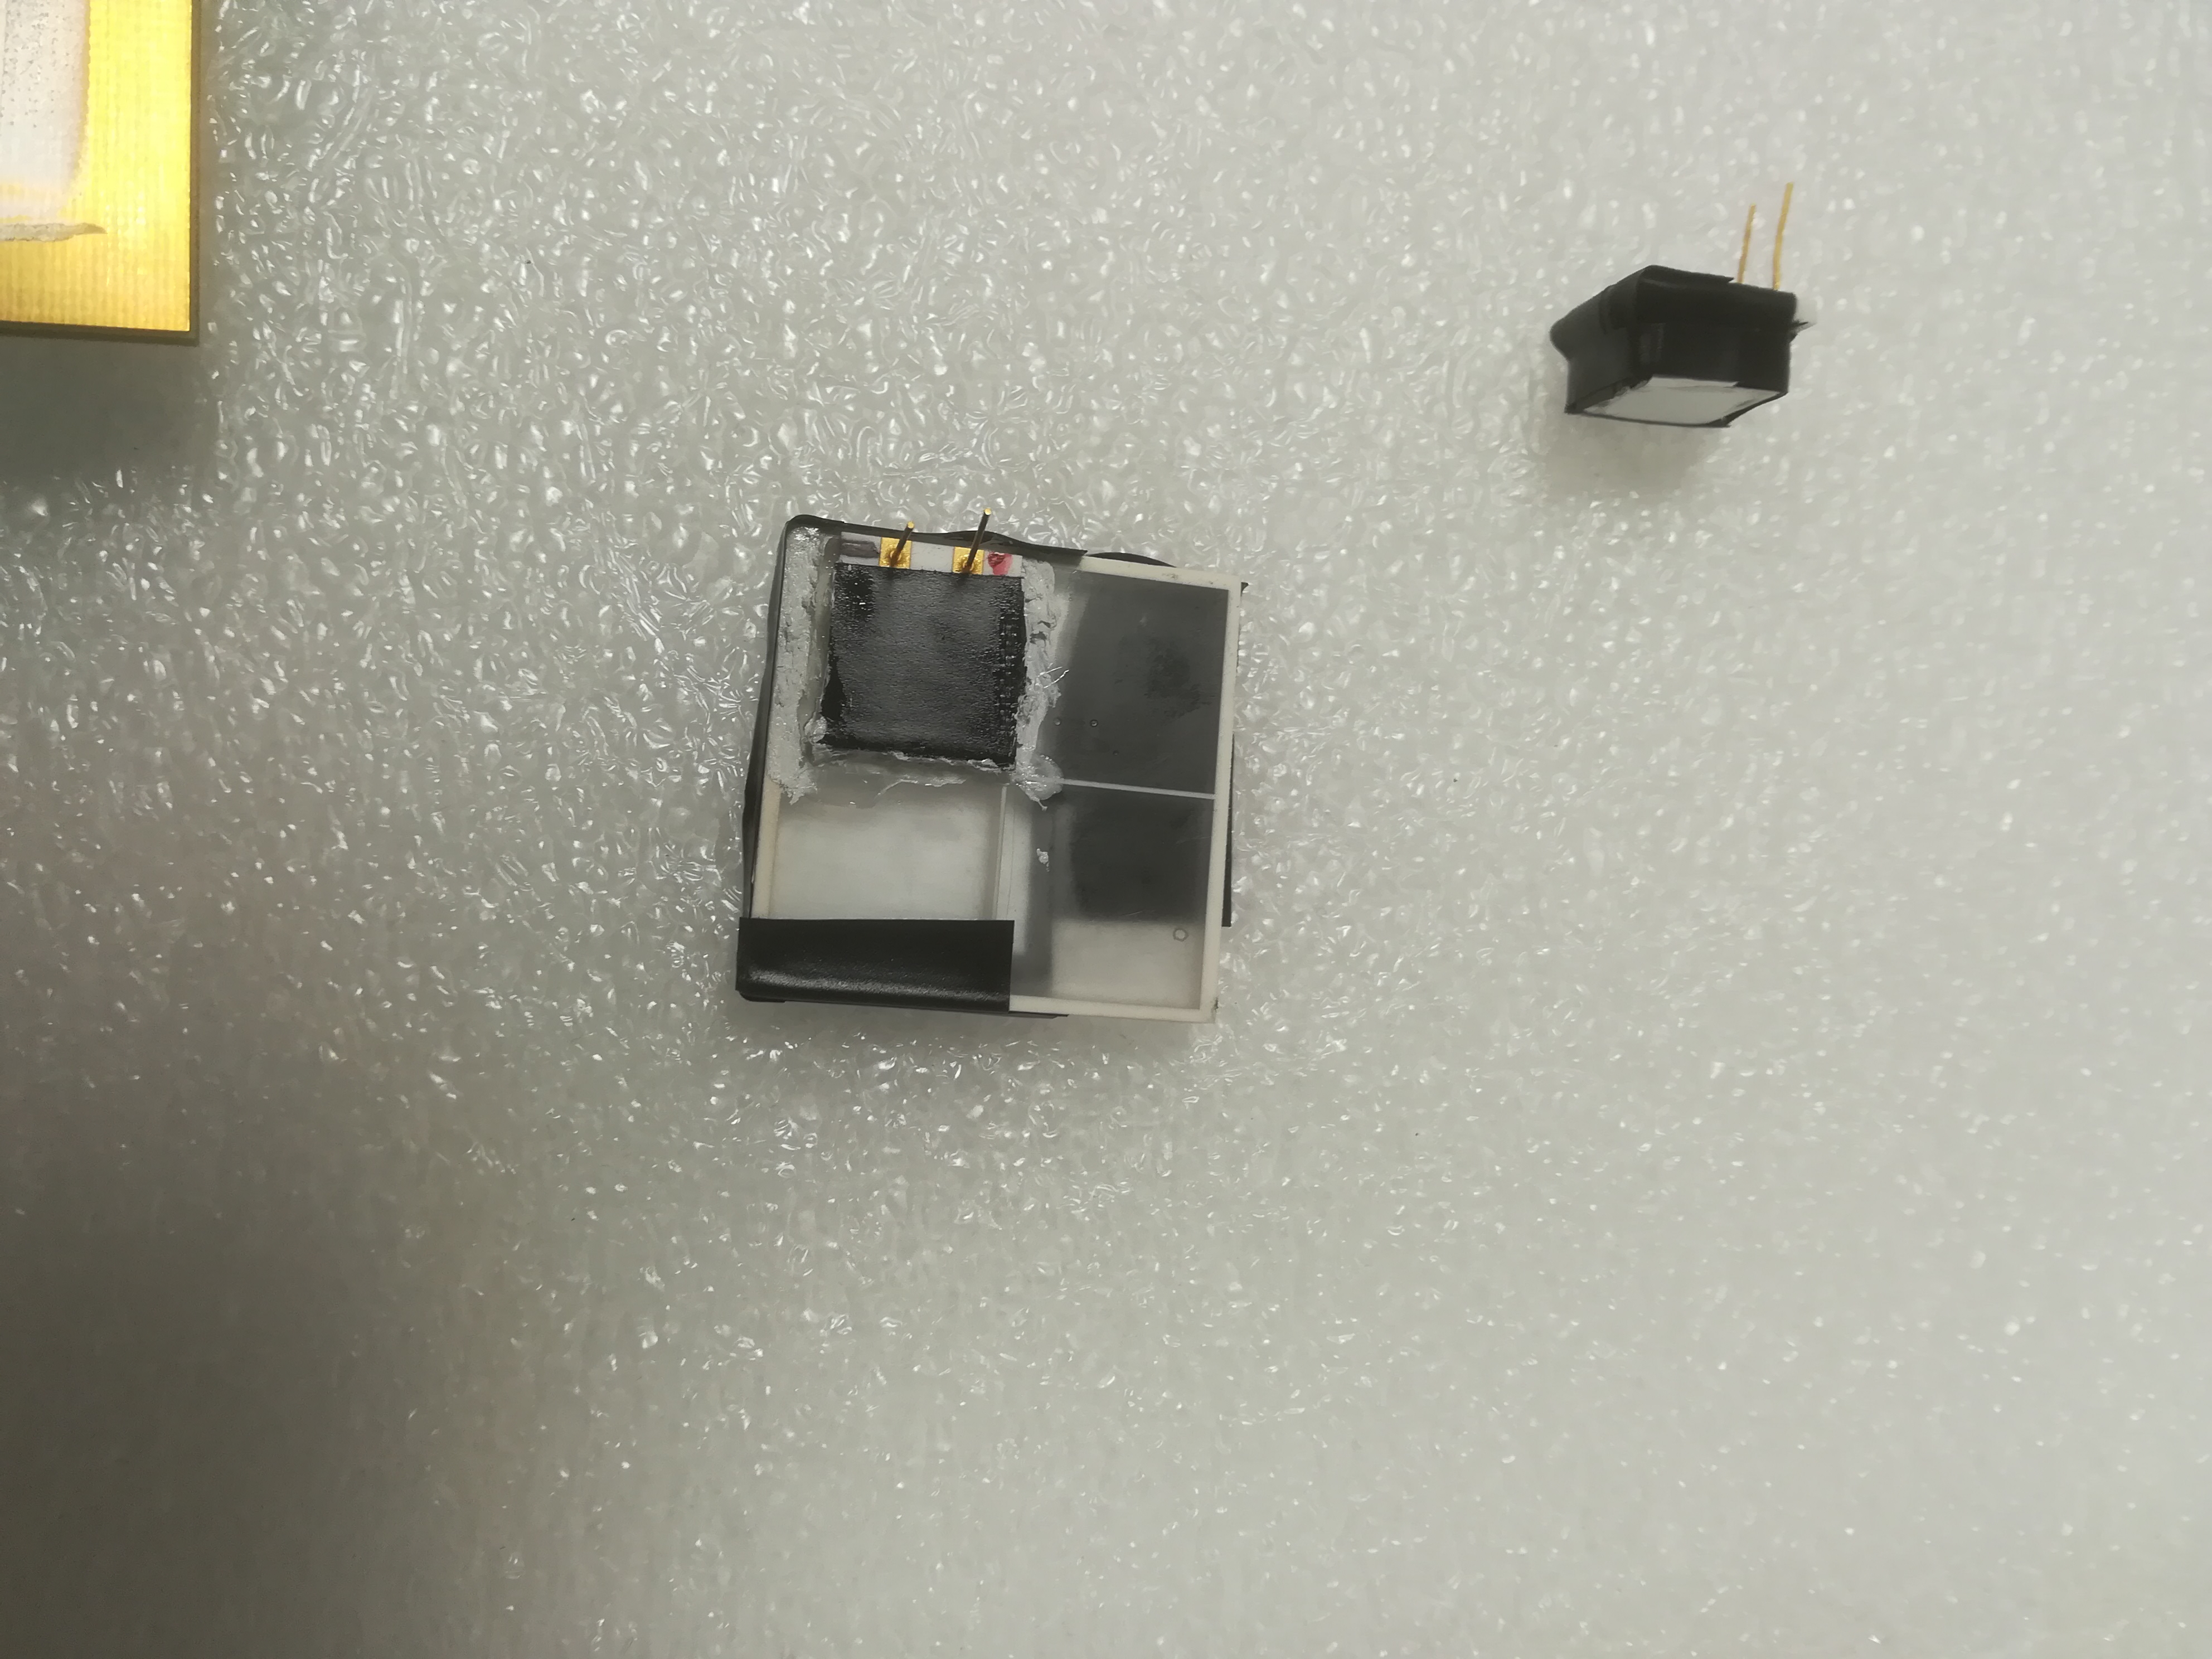
\includegraphics[width=0.48\columnwidth, keepaspectratio]{Grafici_Tesi2/Confronto/csi.png}
%	\end{subfigure}
%\end{figure}\\
%\textit{Confronto tra gli spettri sperimentali~(blu) e quelli simulati~(rosso).}
\begin{figure} [!h]
	\centering
	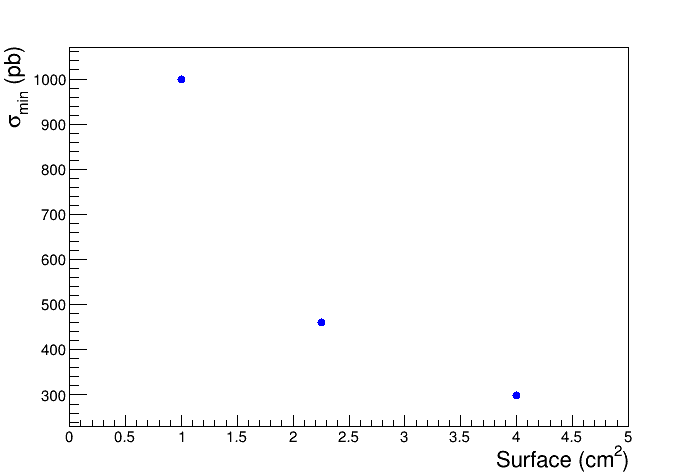
\includegraphics[width=0.7\columnwidth, keepaspectratio]{Grafici_Tesi2/Granularitanew/sigma_min.png}
\end{figure}\\
%\begin{center}
\textit{Andamento della sensibilità di misura $(\sigma_{min})$ al variare della superficie dei telescopi.}\\

\begin{figure} [!h]
	\centering
	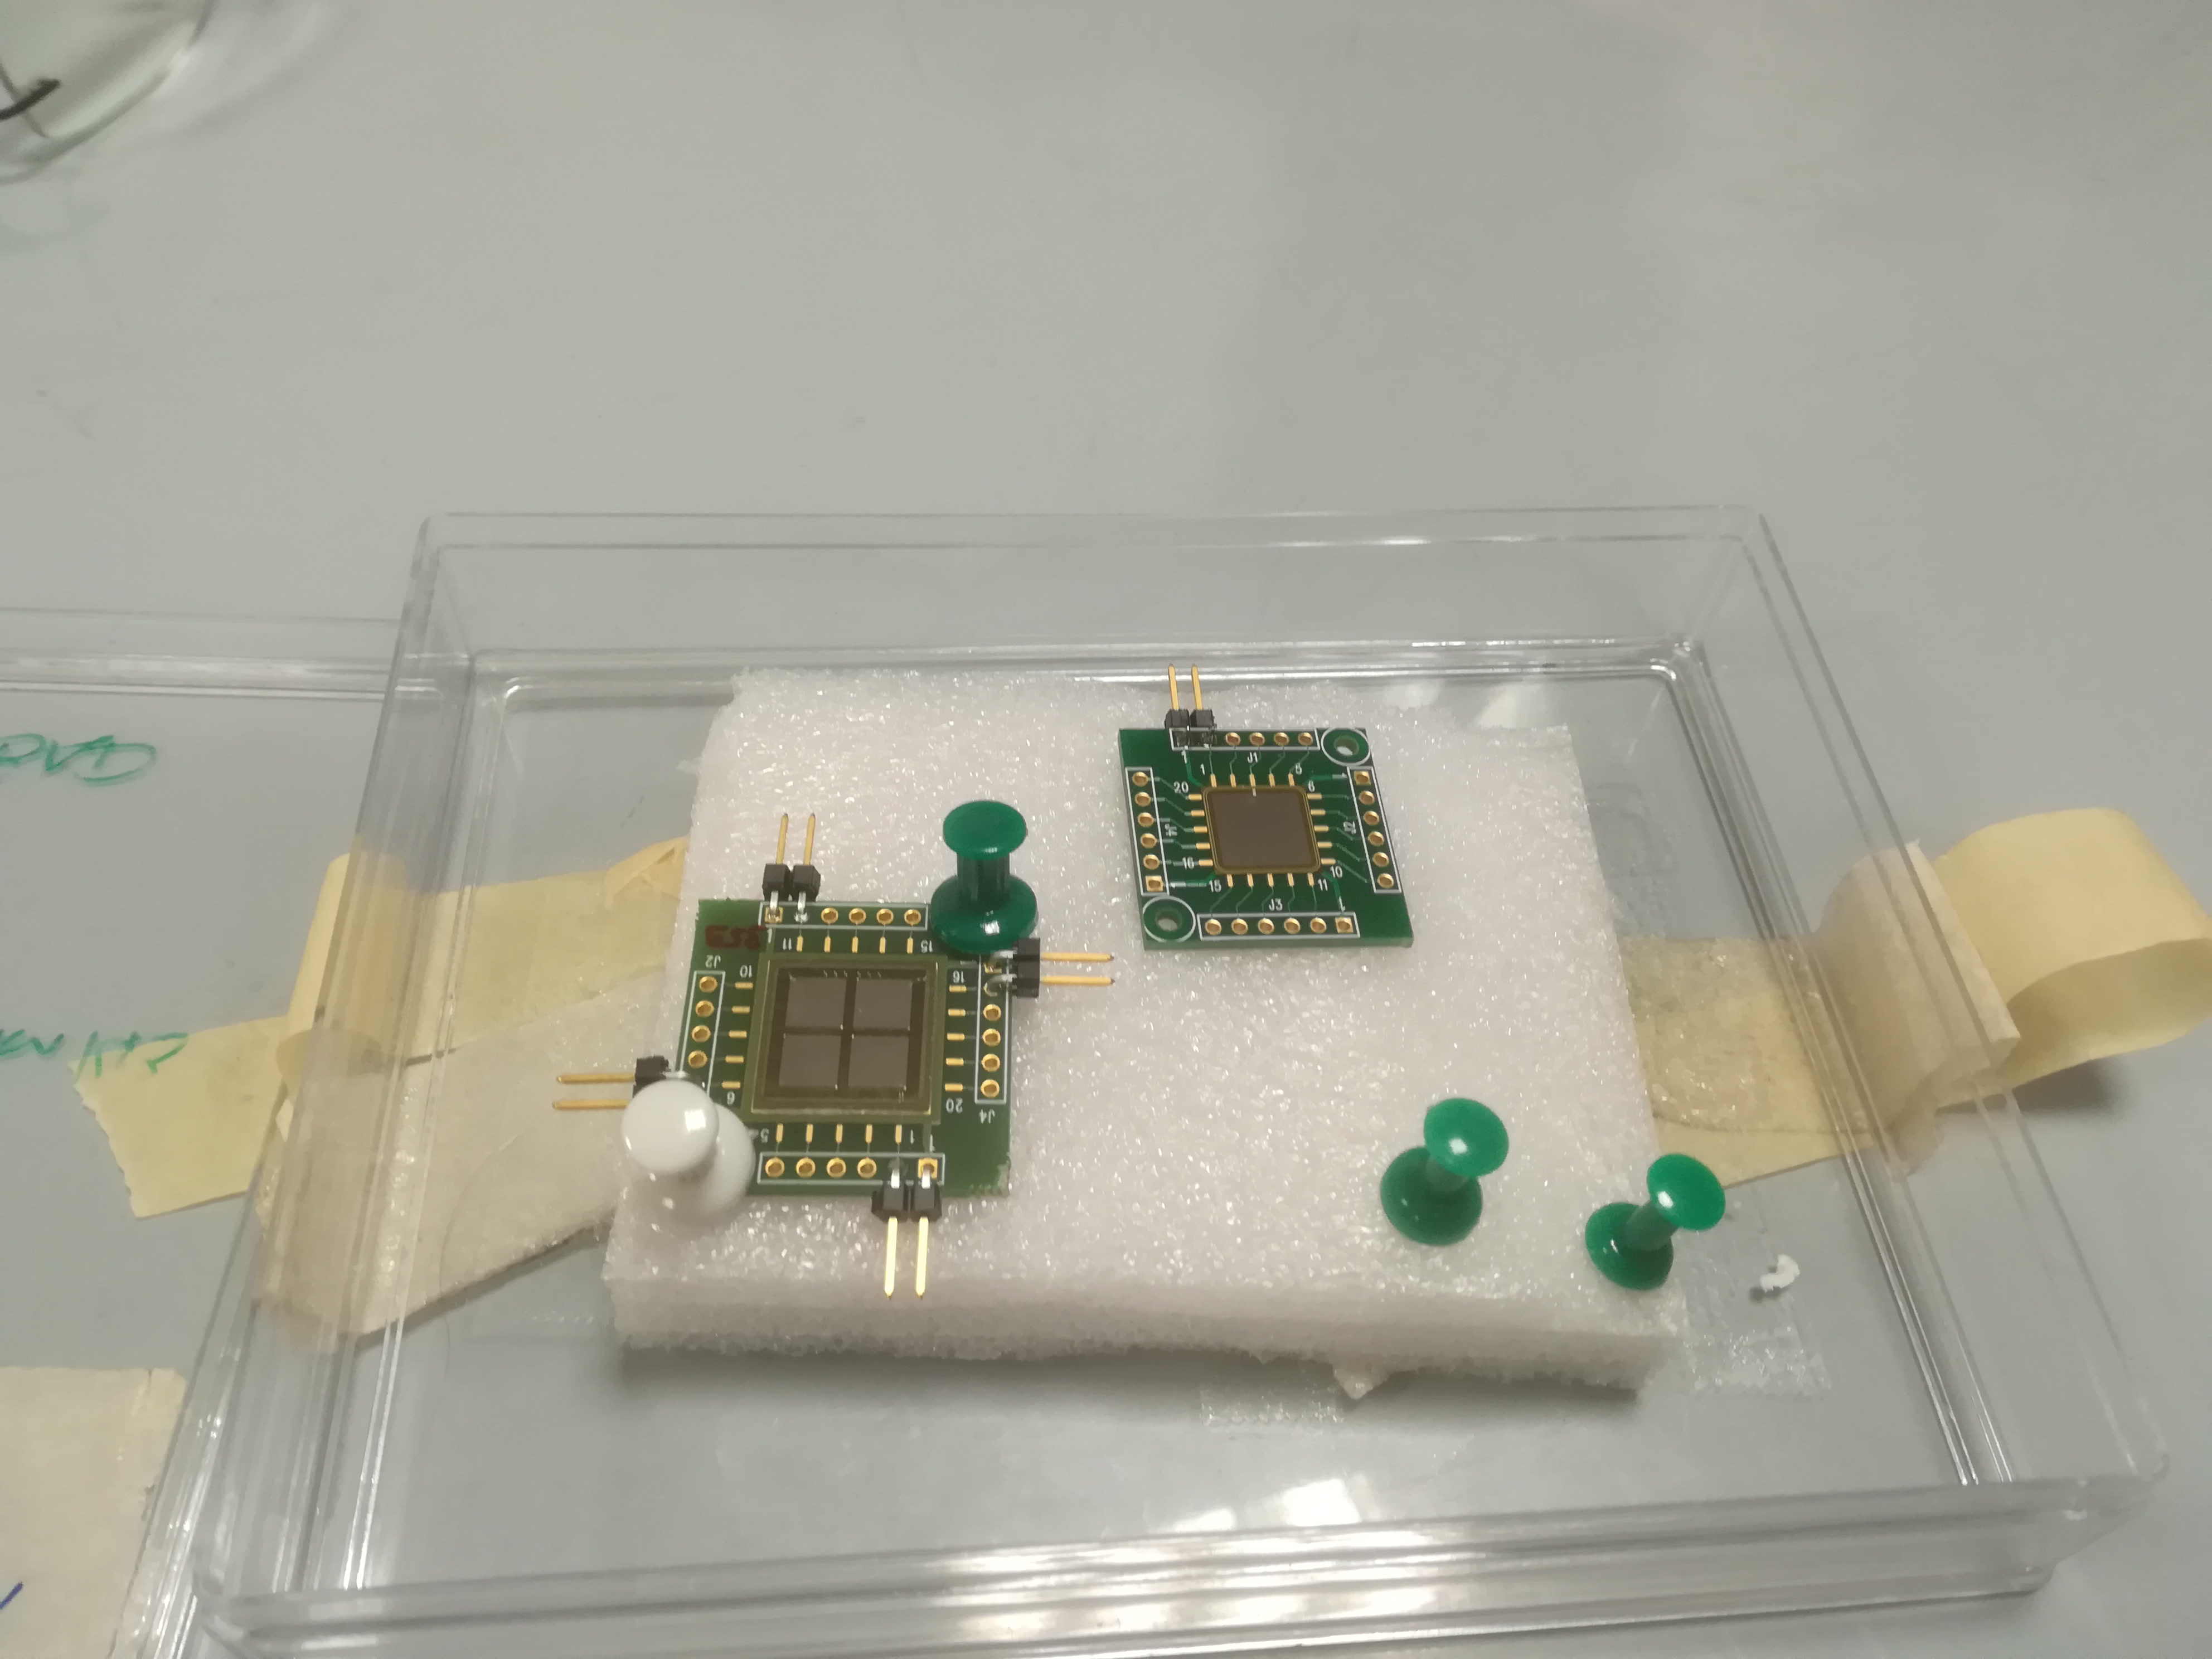
\includegraphics[width=0.75\columnwidth, keepaspectratio]{Grafici_Tesi2/Confronto/sic.png}
\end{figure}
\textit{Spettro in $\Delta E_{SiC}$: in blu quello sperimentale, in rosso quello simulato.}


%\section{Conclusions}
\section{Conclusioni}

%\lipsum[14]

Il tool di simulazioni sviluppato per questo lavoro di tesi ha dimostrato che un sistema di rivelazione basato sulla tecnologia SiC-CsI può garantire le capacità di PID e la sensibilità di misura necessarie per gli scopi del progetto~NUMEN.

Lo studio di diverse condizioni di granularità ha evidenziato che le capacità di PID migliorano all'aumentare della superficie dei telescopi; tuttavia, in condizioni di alti flussi di particelle incidenti bisogna tenere in considerazione anche la probabilità di pile-up, la quale aumenta velocemente al crescere della superficie.
Inoltre, nella scelta della condizione di granularità da adottare entrano in gioco anche altri fattori, legati, ad esempio, al numero totale di dispositivi e al numero di canali necessari per la lettura.
Di conseguenza, bisogna cercare una soluzione di compromesso tra tutte le esigenze; da questo lavoro si può dedurre che tale soluzione è rappresentata dai telescopi da 1.5$\times$1.5~$\mbox{cm}^2$.
%Alla luce di questo accordo è possibile affermare che la simulazione riesce a riprodurre bene la realtà sperimentale, convalidando i risultati ottenuti nel corso di questo lavoro.

Infine, l'accordo tra i dati sperimentali e quelli simulati permette di avvalorare con buona confidenza l'efficacia del tool di simulazioni e dà, dunque, una validazione dei risultati ottenuti.











%\section{Acknowledgements}

%\lipsum[1]

\section{Contatti}

Giuseppe Antonio Brischetto\\ {\tt brischetto.giuseppe@studium.unict.it}

\end{document}
